\documentclass[12pt, a4paper]{article}
\usepackage[margin=0.5in]{geometry}

\usepackage{color}
\usepackage[dvipsnames]{xcolor}
\usepackage{hyperref}
\hypersetup{
    colorlinks=true,
    linkcolor=blue,
    urlcolor=blue,
    linktoc=all
}


\usepackage{amsmath}
\usepackage{mathtools}
\usepackage{amssymb}
\usepackage{cancel}
\usepackage{bm}
\usepackage{dsfont}
\usepackage{graphicx}
\usepackage{graphics}
\usepackage{xfrac}
\usepackage{array}
\setcounter{MaxMatrixCols}{40}

\usepackage{enumerate}
\usepackage{enumitem}
\usepackage{multirow}

%inclusions carried over from past class homework formats
\usepackage{units}
\usepackage{fullpage}
\usepackage{alltt}
\usepackage{mathrsfs}
\usepackage{xcolor}
\usepackage{soul}

\usepackage{pgfplots}

\DeclarePairedDelimiter{\abs}{\lvert}{\rvert}
\newcommand*{\fontCourier}{\fontfamily{pcr}\selectfont}
\newcommand*\mean[1]{\overline{#1}}
\newcommand\scalemath[2]{\scalebox{#1}{\mbox{\ensuremath{\displaystyle #2}}}}

\setcounter{tocdepth}{5}
\setcounter{secnumdepth}{5}

\usepackage{pdfpages}
\usepackage{Sweave}
\begin{document}

\includepdf{TitlePage_MastersThesis}

\includepdf{ThesisApprovalPage}
\Sconcordance{concordance:Thesis.tex:Thesis.Rnw:%
1 49 1 1 0 7 1 1 4 99 1 1 31 1 12 69 1 1 45 1 2 179 1 1 46 1 2 120 1 1 %
23 7 0 1 76 4 0 1 5 32 1 1 26 1 4 26 1}


\tableofcontents
\newpage


%%%%%%%%%%%%%%%%%%%%%%%%%%%%%%%%%
%%INTRODUCTION
%%%%%%%%%%%%%%%%%%%%%%%%%%%%%%%%%
\section{Thesis Abstract}
  \begin{itemize}
    \item (paragraph) Statement of the thesis topic and objectives
    \item (paragraph) Explanation of R package
  \end{itemize}

\clearpage

\section{Introduction:  Predictive Inference}

  \subsection{Why is predictive inference important?}

  \subsection{Difference between parametric inference and predictive inference}

    \subsubsection{When is predictive inference more useful?}

    \subsubsection{When is parametric inference more useful?}
      [examples, comparisons]

  \subsection{The Bayesian Parametric Prediction Format}
    [Geisser p. 49]\\

        Let $$f\left(x^{(N)},x_{(M)}|\theta\right) = f\left(x_{(M)}|x^{(N)},\theta\right)f\left(x^{(N)}|\theta\right).$$

    Here $x^{(N)}$ represents observed events and $x_{(M)}$ are future events.  We calculate

    $$f\left(x_{(M)},x^{(N)}\right) = \int f\left(x^{(N)},x_{(M)}|\theta\right)p(\theta)d\theta$$

    where $p(\theta)$ is the prior density and

    $$f\left(x_{(M)}|x^{(N)}\right) = \frac{f\left(x_{(M)},x^{(N)}\right)}{f\left(x^{(N)}\right)} = \int f\left(x_{(M)}|\theta\right)p\left(\theta|x^{(N)}\right)d\theta$$

    where

    $$p\left(\theta|x^{(N)}\right) \propto f\left(x^{(N)}|\theta\right)p(\theta).$$

  \subsection{[Maybe] Example of Difference between results from Plug-in estimator and results using Predictive Inference}

\clearpage

\section{Chapter 1:  Predictive Problems with Conjugate Priors}

  [Problems with closed-form solutions.  These problems will be what the R package is designed for.  Use problems from Geisser, Casella \& Berger (Bayesian chapter), other sources.  Regression problem--predictive distributions of models that include and exclude some predictor]

  \subsection{Prediction of Future Successes:  Beta-Binomial (Geisser p. 73)}


    \subsubsection{Derivation}

      Let $X_i$ be independent binary variables with Pr$(X_i = 1) = \theta$, and let $T = \sum X_i$.  Then $T$ has probability

      $${N\choose t}\theta^t(1-\theta)^{N-t}.$$

      \vspace{5mm}

      Assume $\theta\sim\text{Beta}(\alpha,\beta)$, so

      \vspace{5mm}

      $$p(\theta) = \frac{\Gamma(\alpha + \beta)\theta^{\alpha - 1}(1 - \theta)^{\beta - 1}}{\Gamma(\alpha)\Gamma(\beta)}.$$

      \vspace{5mm}

      Then

      \vspace{5mm}

      $$p\left(\theta|X^{(N)}\right) = \frac{\Gamma(N+\alpha+\beta)\theta^{t+\alpha-1}(1-\theta)^{N-t+\beta-1}}{\Gamma(t+\alpha)\Gamma(N-t+\beta)}$$

      \vspace{5mm}

      \noindent So for $R = \sum_{i=1}^M X_{N+i}$ we have Beta-Binomial predictive distribution

\begin{flalign*}
  \text{Pr}[R=r|t]
  &= \int {M\choose r}\theta^r(1-\theta)^{M-r}p\left(\theta|X^{(N)}\right)d\theta\\
  &\\
  &= {M\choose r}\int \theta^r(1-\theta)^{M-r}\frac{\Gamma(N+\alpha+\beta)}{\Gamma(t+\alpha)\Gamma(N-t+\beta)}\theta^{t+\alpha-1}(1-\theta)^{N-t+\beta-1}d\theta\\
  &\\
  &= \frac{M!}{r!(M-r)!}\frac{\Gamma(N+\alpha+\beta)}{\Gamma(t+\alpha)\Gamma(N-t+\beta)}\int\theta^{r+t+\alpha-1}(1-\theta)^{M-r+N-t+\beta-1}d\theta\\
  &\\
  &= \frac{\Gamma(M+1)\Gamma(N+\alpha+\beta)\Gamma(r+t+\alpha)\Gamma(M-r+N-t+\beta)}{\Gamma(r+1)\Gamma(M-r+1)\Gamma(t+\alpha)\Gamma(N-t+\beta)\Gamma(M+N+\alpha+\beta)}
\end{flalign*}

\clearpage

    \subsubsection{R Implementation}

This result has been used to create ``standard" R functions dpredBB(), ppredBB(), and rpredBB() for the Beta-Binomial distribtuion for density, cumulative probability, and random sampling, respectively (see appendix).  These functions are exercised in the following example.


    \subsubsection{Example}

Suppose $t=5$ successes have been observed out of $N=10$ binary events, $\alpha = 2$ and $\beta = 8$.  For $M = 1000$ future observations, the figures below show the predictive distribution from dpredBB(), the cumulative distribution from ppredBB(), and a histogram of random draws from rpredBB().


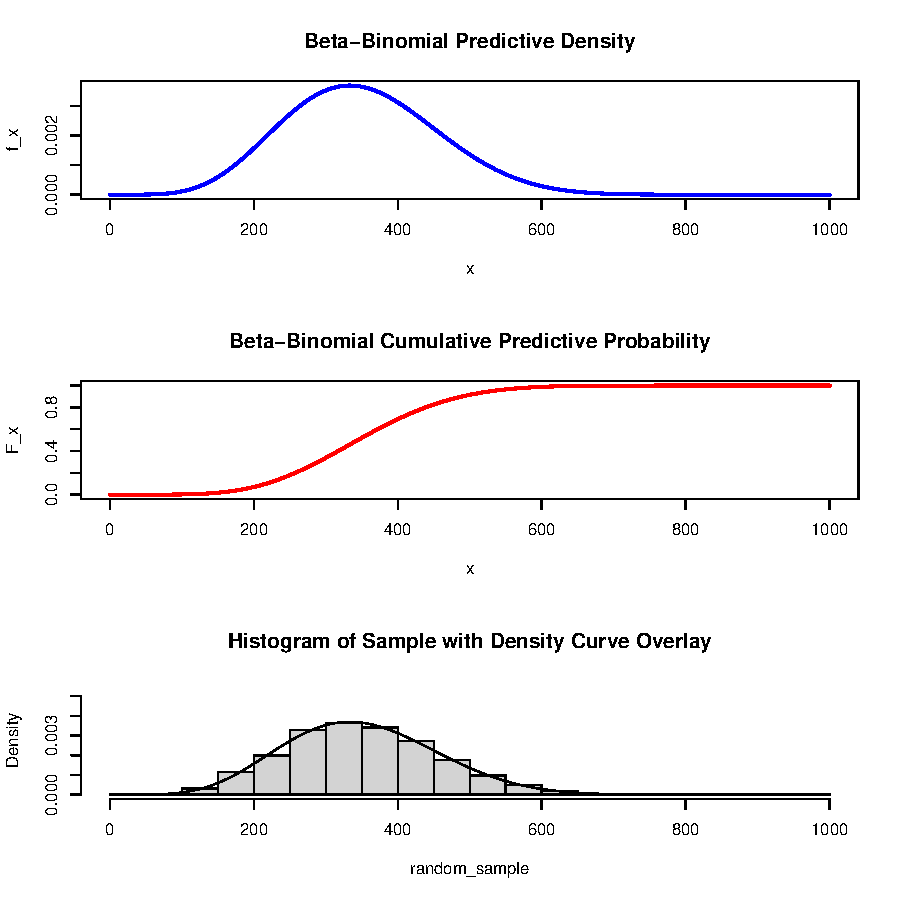
\includegraphics{Thesis-002}



    \subsection{Survival Time:  Exponential-Gamma (Geisser p. 74)}


    \subsubsection{Derivation}

      Suppose $X^{(N)} = \left(X^{(d)},X^{(N-d)}\right)$ where $X^{(d)}$ represents copies fully observed from an exponential survival time density
          $$f(x|\theta) = \theta e^{-\theta x}$$
      and $X^{(N-d)}$ represents copies censored at $x_{d+1},...,x_N$, respectively.  Hence
          $$L(\theta)\propto\theta^d e^{-\theta N\bar{x}}$$
      when $N\bar{x} = \sum_1^N{x_i}$, as shown below.\\

      The usual exponential likelihood is used for the fully observed copies, whereas for the censored copies we need Pr$(x > \theta) = 1 - \text{Pr}(x\leq\theta) = 1 - F(x|\theta) = 1 - (1 - e^{-\theta x}) = e^{-\theta x}$.  Thus the overall likelihood is

      $$L(\theta|x) = \prod_{i=1}^d\theta e^{-\theta x_i}\prod_{i=d+1}^N e^{-\theta x_i} = \theta^d e^{-\theta N\bar{x}}$$

      Assuming a Gamma$(\delta,\gamma)$ prior for $\theta$,

       $$p(\theta) = \frac{\gamma^\delta\theta^{\delta - 1}e^{-\gamma\theta}}{\Gamma(\delta)}$$

       we obtain the posterior

       %$$p\left(\theta|X^{(N)}\right) = \frac{p\left(x^{(N)}|\theta\right)p(\theta)}{\int p\left(X^{(N)}|\theta\right)p(\theta)d\theta} = \frac{(\gamma+N\bar{x})^{d+\delta}\theta^{d+\delta - 1}e^{-\theta(\gamma+N\bar{x})}}{\Gamma(d+\delta)}$$

        \begin{flalign*}
          p\left(\theta|X^{(N)}\right)
          &= \frac{p\left(x^{(N)}|\theta\right)p(\theta)}{\int p\left(X^{(N)}|\theta\right)p(\theta)d\theta}\\
          &\\
          &= \frac{\theta^d e^{-\theta N\bar{x}}\cdot\frac{\gamma^\delta\theta^{\delta - 1}e^{-\gamma\theta}}{\Gamma(\delta)}}{\int\left(\theta^d e^{-\theta N\bar{x}}\cdot\frac{\gamma^\delta\theta^{\delta - 1}e^{-\gamma\theta}}{\Gamma(\delta)}\right)d\theta}\\
          &\\
          &= \frac{\cancel{\frac{\gamma^\delta}{\Gamma(\delta)}}\left(\theta^{d+\delta - 1}e^{-\theta(\gamma+N\bar{x})}\right)}{\cancel{\frac{\gamma^\delta}{\Gamma(\delta)}}\int\left(\theta^{d+\delta - 1}e^{-\theta(\gamma+N\bar{x})}\right)d\theta}\\
          &\\
          &= \frac{\frac{(\gamma+N\bar{x})^{d+\delta}}{\Gamma(d+\delta)}\left(\theta^{d+\delta - 1}e^{-\theta(\gamma+N\bar{x})}\right)}{\cancel{\frac{(\gamma+N\bar{x})^{d+\delta}}{\Gamma(d+\delta)}\int\left(\theta^{d+\delta - 1}e^{-\theta(\gamma+N\bar{x})}\right)d\theta}}\\
          &\\
          &= \frac{(\gamma+N\bar{x})^{d+\delta}\theta^{d+\delta - 1}e^{-\theta(\gamma+N\bar{x})}}{\Gamma(d+\delta)}
        \end{flalign*}

    with the Gamma$(d+\delta,\gamma+N\bar{x})$ density in the next to last step integrating to $1$.\\

    Thus the survival time predictive probability is

    \begin{flalign*}
      P\left(X = x|\theta,X^{(N)}\right)
      &= \int p\left(\theta|X^{(N)}\right)p(x|\theta)d\theta\\
      &\\
      &= \int\frac{(\gamma+N\bar{x})^{d+\delta}\theta^{d+\delta - 1}e^{-\theta(\gamma+N\bar{x})}}{\Gamma(d+\delta)}\cdot\theta e^{-\theta x}d\theta\\
      &\\
      &= (d+\delta)(\gamma+N\bar{x})^{d+\delta}\int\frac{\theta^{(d+\delta + 1) - 1}e^{-\theta(\gamma+N\bar{x} + x)}}{(d+\delta)\Gamma(d+\delta)}d\theta\\
      &\\
      &= \frac{(d+\delta)(\gamma+N\bar{x})^{d+\delta}}{\left(\gamma+N\bar{x}+x\right)^{d+\delta+1}}\int\frac{\left(\gamma+N\bar{x}+x\right)^{d+\delta+1}\theta^{(d+\delta + 1) - 1}e^{-\theta(\gamma+N\bar{x} + x)}}{\Gamma(d+\delta+1)}d\theta\\
      &\\
      &= \frac{(d+\delta)(\gamma+N\bar{x})^{d+\delta}}{\left(\gamma+N\bar{x}+x\right)^{d+\delta+1}}
    \end{flalign*}

    (simplifying by constructing a Gamma$(d+\delta+1,\gamma+N\bar{x}+x)$ density in the final integrand.)\\



    \subsubsection{R Implementation}

This result has been used to create standard format R functions dpredEG(), ppredEG(), and rpredEG() for the Gamma-Exponential distribtuion for density, cumulative probability, and random sampling, respectively (see appendix).  These functions are exercised in the following example.


    \subsubsection{Example}

Suppose $d=800$ out of $N = 1000$ copies have been observed, and the remaining $200$ censored.  Say $\delta = 20$, $\gamma=5$, and we are interested in the number of survivors out of $M = 1000$ future observations.  The figures below illustrate the predictive probability using dpredEG() and rpredEG(), along with a histogram of a random sample taken using rpredEG().


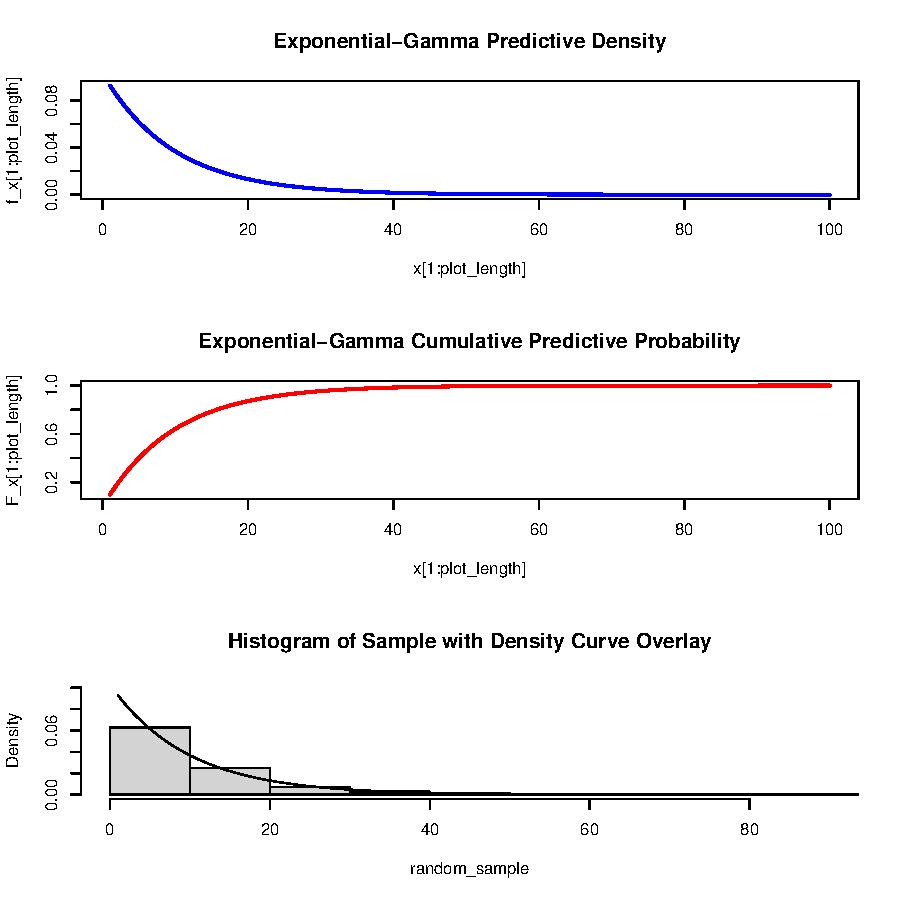
\includegraphics{Thesis-003}

\clearpage

  \subsection{Poisson-Gamma Model (Hoff p. 43ff)}
    \subsubsection{Derivation}
    [using Hoff's notation and variable names below.  Should I convert this to Geisser's $x^{(N)},x_{(M)}$ convention for uniformity throughout my thesis?]\\\\
      Suppose $Y_1,...,Y_n|\theta\overset{i.i.d.}{\sim}\text{Poisson}(\theta)$ with Gamma prior $\theta\sim\text{Gamma}(\alpha,\beta)$.  That is,

      \begin{flalign*}
        P\left(Y_1 = y_1,...,Y_n = y_n|\theta\right)
        &= \prod_{i=1}^n p\left(y_i|\theta\right)\\
        &\\
        &= \prod_{i=1}^n\frac{1}{y!}\theta^{y_i}e^{-\theta}\\
        &\\
        &= \left(\prod_{i=1}^n\frac{1}{y!}\right)\theta^{\sum y_i}e^{-n\theta}\\
        &\\
        &= c\left(y_1,...,y_n\right)\theta^{\sum y_i}e^{-n\theta}
      \end{flalign*}

      and

      $$p(\theta) = \dfrac{\beta^\alpha}{\Gamma(\alpha)}\theta^{\alpha-1}e^{-\beta\theta}, \theta, \alpha, \beta > 0.$$

\bigskip

      Then we have posterior distribution

      \begin{flalign*}
        p\left(\theta|y_1,...,y_n\right)
        &= \dfrac{p\left(y_1,...,y_n|\theta\right)p(\theta)}{\int_\theta p\left(y_1,...,y_n|\theta\right)p(\theta)}\\
        &\\
        &= \dfrac{p\left(y_1,...,y_n|\theta\right)p(\theta)}{p\left(y_1,...,y_n\right)}\\
        &\\
        &= \dfrac{1}{p\left(y_1,...,y_n\right)}\theta^{\sum y_i}e^{-n\theta}\dfrac{\beta^\alpha}{\Gamma(\alpha)}\theta^{\alpha - 1}e^{-\beta\theta}\\
        &\\
        &= C\left(y_1,...,y_n,\alpha,\beta\right)\theta^{\alpha+\sum y_i - 1}e^{-(\beta + n)\theta}\\
        &\\
        &\sim \text{Gamma}\left(\alpha+\sum y_i,\beta + n\right).
      \end{flalign*}


      Here

      \begin{flalign*}
        C\left(y_1,...,y_n,\alpha,\beta\right)
        &= \dfrac{1}{p\left(y_1,...,y_n\right)}\cdot\dfrac{\beta^\alpha}{\Gamma(\alpha)}\\
        &\\
        &= \dfrac{1}{\int_\theta p\left(y_1,...,y_n|\theta\right)p(\theta)}\cdot\dfrac{\beta^\alpha}{\Gamma(\alpha)}\\
        &\\
        &= \dfrac{1}{\int_\theta\left(\prod\frac{1}{y_i!}\right)\theta^{\sum y_i}e^{-n\theta}\cancel{\left(\frac{\beta^\alpha}{\Gamma(\alpha)}\right)}\theta^{\alpha-1}e^{-\beta\theta}}\cdot\cancel{\left(\frac{\beta^\alpha}{\Gamma(\alpha)}\right)}
        &\\
        &= \dfrac{1}{\left(\prod\frac{1}{y_i!}\right)\frac{\Gamma(\alpha + \sum y_i)}{(\beta+n)^{\alpha+\sum y_i}}\int_\theta \frac{(\beta+n)^{\alpha+\sum y_i}}{\Gamma(\alpha+\sum y_i)}\theta^{\sum y_i+\alpha-1}e^{-(\beta+n)\theta}}\\
        &\\
        &= \dfrac{\prod_{i=1}^n y_i!(\beta+n)^{\alpha+\sum y_i}}{\Gamma(\alpha+\sum y_i)}
      \end{flalign*}

      Call this constant $C_n$ (for $n$ observations).

\bigskip

      Note that an additional observation $y_{n+1} = \tilde{y}$ the constant becomes

      $$C_{n+1} = \dfrac{\prod_{i=1}^{n+1} y_i!(\beta+n+1)^{\alpha+\sum_{i=1}^{n+1} y_i}}{\Gamma(\alpha+\sum_{i=1}^{n+1} y_i)}.$$

      Also note that the marginal joint distribution of $k$ observations is

      $$p\left(\tilde{y}|y_1,...,y_k\right) = \dfrac{1}{C_k}\dfrac{\beta^\alpha}{\Gamma(\alpha)}.$$

      For future observation $\tilde{y}$, then, we compute predictive distribution

      \begin{flalign*}
        p\left(\tilde{y}|y_1,...,y_n\right)
        &= \dfrac{p\left(y_1,...,y_n,\tilde{y}\right)}{p\left(y_1,...,y_n\right)} = \dfrac{p\left(y_1,...,y_{n+1}\right)}{p\left(y_1,...,y_n\right)}
        = \dfrac{\frac{1}{C_{n+1}}\cancel{\frac{\beta^\alpha}{\Gamma(\alpha)}}}{\frac{1}{C_n}\cancel{\frac{\beta^\alpha}{\Gamma(\alpha)}}}
        = \dfrac{C_n}{C_{n+1}}\\
        &\\
        &= \dfrac{\dfrac{\prod_{i=1}^n y_i!(\beta+n)^{\alpha+\sum_{i=1}^n y_i}}{\Gamma(\alpha+\sum_{i=1}^n y_i)}}{\dfrac{\prod_{i=1}^{n+1} y_i!(\beta+n+1)^{\alpha+\sum_{i=1}^{n+1} y_i}}{\Gamma(\alpha+\sum_{i=1}^{n+1} y_i)}}\\
        &\\
        &= \dfrac{\Gamma\left(\alpha+\sum_{i=1}^{n+1}y_i\right)(\beta+n)^{\alpha+\sum_{i=1}^n y_i}}{\left(y_{n+1}!\right)\Gamma\left(\alpha+\sum_{i=1}^n y_i\right)(\beta+n+1)^{\alpha+\sum_{i=1}^{n+1}y_i}}\\
        &\\
        &= \dfrac{\Gamma\left(\alpha+\sum_{i=1}^n y_i + \tilde{y}\right)(\beta+n)^{\alpha+\sum_{i=1}^n y_i}}{\left(\tilde{y}!\right)\Gamma\left(\alpha+\sum_{i=1}^n y_i\right)(\beta+n+1)^{\alpha+\sum_{i=1}^n y_i + \tilde{y}}}\\
        &\\
        &= \dfrac{\Gamma\left(\alpha+\sum y_i+\tilde{y}\right)}{\Gamma(\tilde{y}+1)\Gamma(\alpha+\sum y_i)}\cdot \left(\dfrac{\beta+n}{\beta+n+1}\right)^{\alpha+\sum y_i} \cdot \left(\dfrac{1}{\beta+n+1}\right)^{\tilde{y}}\\
      \end{flalign*}

This is a negative binomial distribution:  $\tilde{y}\sim NB\left(\alpha+\sum y_i,\beta+n\right)$, for which

\begin{flalign*}
  E\left[\tilde{Y}|y_1,...,y_n\right] &= \dfrac{a+\sum{y_i}}{b+n} = E\left[\theta|y_1,...,y_n\right];\\
  &\\
  \text{Var}\left[\tilde{Y}|y_1,...,y_n\right] &= \dfrac{a+\sum{y_i}}{b+n}\dfrac{b+n+1}{b+n}\\
  &\\
  &=\text{Var}\left[\theta|y_1,...,y_n\right]\times(b+n+1)\\
  &\\
  &=E\left[\theta|y_1,...,y_n\right]\times\dfrac{b+n+1}{b+n}\\
\end{flalign*}

\vspace{5mm}

\hrule

\vspace{5mm}

[Showing here that it is indeed a NB distribution]

$$\theta\sim NB(\alpha,\beta)\Rightarrow p(\theta) = \binom{\theta+\alpha-1}{\alpha - 1}\left(\dfrac{\beta}{\beta+1}\right)^\alpha\left(\dfrac{1}{\beta+1}\right)^\theta$$

\begin{center}so\end{center}

\begin{flalign*}
  \tilde{y}\sim NB\left(\alpha + \sum{y_i}),\beta+n\right)\Rightarrow p(\tilde{y})
  &= \binom{\tilde{y}+\alpha+\sum{y_i}-1}{\alpha+\sum{y_i}-1}\left(\dfrac{\beta+n}{\beta+n+1}\right)^{\alpha+\sum{y_i}}\left(\dfrac{1}{\beta+n+1}\right)^{\tilde{y}}\\
  &\\
  &= \dfrac{\left(\alpha + \sum{y_i} + \tilde{y} - 1\right)!}{\left(\alpha + \sum{y_i} - 1\right)!\left(\tilde{y}\right)!}\left(\dfrac{\beta+n}{\beta+n+1}\right)^{\alpha+\sum{y_i}}\left(\dfrac{1}{\beta+n+1}\right)^{\tilde{y}}\\
  &\\
  &= \dfrac{\Gamma\left(\alpha + \sum{y_i} + \tilde{y}\right)}{\Gamma\left(\alpha + \sum{y_i}\right)\Gamma\left(\tilde{y}+1\right)}\left(\dfrac{\beta+n}{\beta+n+1}\right)^{\alpha+\sum{y_i}}\left(\dfrac{1}{\beta+n+1}\right)^{\tilde{y}}
\end{flalign*}

\vspace{5mm}

\hrule

\vspace{5mm}

      \bigskip



      [This is the result in Hoff.  The straightforward derivation below is off by a constant multiple.  Need to figure out what went awry.]



      \begin{flalign*}
        p\left(\tilde{y}|y_1,...,y_n\right)
        &= \int_0^\infty p\left(\tilde{y}|\theta,y_1,...,y_n\right)p\left(\theta|y_1,...,y_n\right)d\theta\\
        &\\
        &= \int p\left(\tilde{y}|\theta\right)p\left(\theta|y_1,...,y_n\right)d\theta\\
        &\\
        &= C\int\left(\dfrac{1}{\tilde{y}!}\theta^{\tilde{y}}e^{-\theta}\right)\theta^{\alpha+\sum y_i - 1}e^{-(\beta+n)\theta}d\theta\\
        &\\
        &= \dfrac{C}{\tilde{y}!}\int\theta^{\tilde{y}+\alpha+\sum y_i - 1}e^{-(\beta+n+1)\theta}d\theta\\
        &\\
        &= \dfrac{C\Gamma\left(\tilde{y}+\alpha+\sum y_i\right)}{\Gamma\left(\tilde{y}+1\right)(\beta+n+1)^{\tilde{y}+\alpha+\sum y_i}}\int\dfrac{(\beta+n+1)^{\tilde{y}+\alpha+\sum y_i}}{\Gamma\left(\tilde{y}+\alpha+\sum y_i\right)}\theta^{\tilde{y}+\alpha+\sum y_i - 1}e^{-(\beta+n+1)\theta)}d\theta\\
        &\\
        &= C\cdot\dfrac{\Gamma\left(\tilde{y}+\alpha+\sum y_i\right)}{\Gamma\left(\tilde{y}+1\right)(\beta+n+1)^{\tilde{y}+\alpha+\sum y_i}}\\
        &\\
        &= \dfrac{\prod_{i=1}^n y_i!(\beta+n)^{\alpha+\sum y_i}}{\Gamma(\alpha+\sum y_i)}\cdot\dfrac{\Gamma\left(\tilde{y}+\alpha+\sum y_i\right)}{\Gamma\left(\tilde{y}+1\right)(\beta+n+1)^{\tilde{y}+\alpha+\sum y_i}}\\
        &\\
        &= \prod_{i=1}^n y_i! \cdot \dfrac{\Gamma\left(\tilde{y}+\alpha+\sum y_i\right)}{\Gamma(\tilde{y}+1)\Gamma(\alpha+\sum y_i)}\cdot \left(\dfrac{\beta+n}{\beta+n+1}\right)^{\alpha+\sum y_i} \cdot \left(\dfrac{1}{\beta+n+1}\right)^{\tilde{y}}\\
      \end{flalign*}

\textcolor{red}{Hoff p.47:
  \begin{itemize}
    \item $b$ is interpreted as the number of prior observations
    \item $a$ is interpreted as the sum of counts from $b$ prior observations
  \end{itemize}
}

\textcolor{red}{  Hoff p. 49 (Birth rate example):  $a = 2, b = 1$. }


    \subsubsection{R Implementation}

This result has been used to create standard format R functions dpredPG(), ppredPG(), and rpredPG() for the Poisson-Gamma distribution for density, cumulative probability, and random sampling, respectively (see appendix).  These functions are exercised in the following example.\\

    Developing the random sample function rpredPG():  I need to establish the support of the predictive distribution $f_x$ from which to sample.  the uniroot() function is not working because it keeps feeding non-integer values to dnbinom().  Strategy: a modified bisection method as follows:\\

    \begin{enumerate}
      \item set a desired tolerance $\epsilon$.
      \item Find the expected value $E_x$ (closed formula, see above).
      \item Step to the right of $E_x$ by whole integers, in the sequence $E_x + \{1,2,4,...2^n\}$, stopping at $U=f_x\left(E_x + 2^n\right) < 0$.  This is the upper bound for the bisection method.
      \item Bisect the interval, rounding to the nearest integer.  Call the resulting mid-interval number $B$.
      \item If B is positive, test whether $0 \leq f_x(B) \leq \epsilon$.  If so, DONE.  If not:
      \item Establish new interval, choosing endpoints from $E_x$, $B$, and $U$ so that the interval straddles $0$, and repeat the steps until the condition in step 5 is reached.
    \end{enumerate}

    \subsubsection{Example}

Suppose we have 10 prior observations with counts 27, 79, 21, 100, 8, 4, 37, 15, 3, 97.  Let $\alpha = 11$ and $\beta = 3$.  For $\tilde{y} = 1:100$ possible future occurrences, the figures below show the predictive distribution from dpredPG(), the cumulative distribution from ppredPG(), and a histogram of random draws from rpredPG().

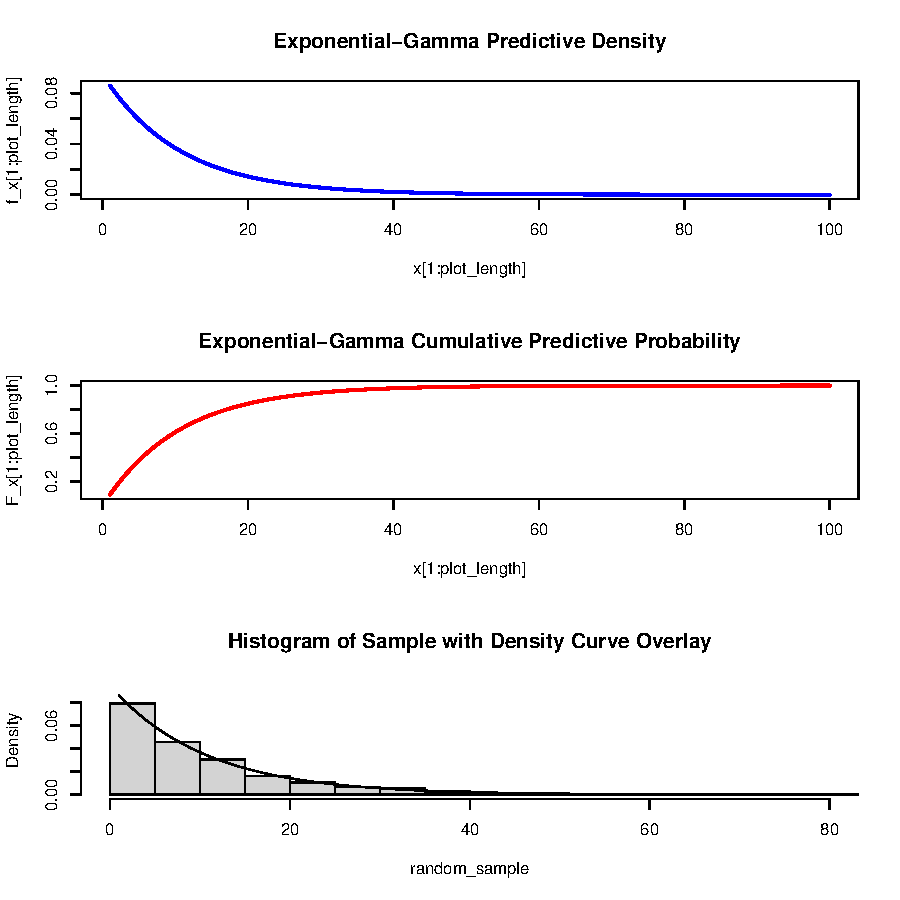
\includegraphics{Thesis-004}

\clearpage

  \subsection{Normal Observation with Normal-Inverse Gamma Prior}
    \subsubsection{One sample}
      \paragraph{Derivation}
      [Hoff p. 69ff]\\
        Let $\left\{Y_1,...,Y_n|\theta,\sigma^2\right\}\overset{i.i.d.}{\sim}N\left(\theta,\sigma^2\right)$.  Then the joint sampling density is

        \begin{flalign*}
          p\left(y_1,...,y_n|\theta,\sigma^2\right)
          &= \prod_{i=1}^n p\left(y_i|\theta,\sigma^2\right)\\
          &\\
          &= \prod_{i=1}^n \dfrac{1}{\sqrt{2\pi\sigma^2}}e^{-\frac{1}{2}\left(\frac{y_i - \theta}{\sigma}\right)^2}\\
          &\\
          &= \left(2\pi\sigma^2\right)^{-\sfrac{n}{2}}e^{-\frac{1}{2}\sum_{i=1}^n\left(\frac{y_i - \theta}{\sigma}\right)^2}.\\
        \end{flalign*}

        %It can be shown that $\left\{\sum{y_i^2},\sum{y_i}\right\}$ and hence $\left\{\bar{y},s^2\right\}$ are sufficient statistics, where $\bar{y} = \sum{y_i}/n$ and $s^2 = \sum\left(y_i - \bar{y}\right)^2/(n-1)$.\\


        %\vdots

        Following Hoff (p. 74ff), for joint inference on both $\theta$ and $\sigma$, assume priors

        \begin{flalign*}
          \frac{1}{\sigma^2} &\sim \text{gamma}\left(\sfrac{\nu_0}{2},\sfrac{\nu_0\sigma_0^2}{2}\right)\\
          &\\
          \theta|\sigma^2 &\sim \text{normal}\left(\mu_0,\sfrac{\sigma^2}{\kappa_0}\right)\\
        \end{flalign*}

        where $\left(\sigma_0^2,\nu_0\right)$ are the sample variance and sample size of prior observations, and $\left(\mu_o, \kappa_0\right)$ are the sample mean and sample size of prior observations.\\

        Note:  $\mu_0$, $\kappa_0$, $\nu_0$, and $\sigma_0^2$ come from prior knowledge. [in the Hoff example (Midge Wing Length), $\kappa_0$ and $\nu_0$ are both set to $1$ so that ``our prior distributions are only weakly centered around these estimates from other populations."]\\

        From this we derive joint posterior distribution

        \begin{flalign*}
          \left\{\theta|y_1,...,y_n,\sigma^2\right\} &\sim \text{normal}\left(\mu_n,\sfrac{\sigma^2}{\kappa_n}\right)\\
          &\\
          \left\{\sigma^2|y_1,...,y_n\right\} &\sim \text{inverse-gamma}\left(\sfrac{\nu_n}{2},\sfrac{\sigma^2_n\nu_n}{2}\right).
        \end{flalign*}

        where

        \begin{flalign*}
          \kappa_n &= \kappa_0 + n\\
          &\\
          \mu_n &= \frac{\kappa_0\mu_0+n\bar{y}}{\kappa_n}\\
          &\\
          \nu_n &= \nu_0 + n\\
          &\\
          \sigma_n^2 &= \frac{1}{\nu_n}\left[\nu_0\sigma_0^2 + (n-1)s^2 + \frac{\kappa_0 n}{\kappa_n}\left(\bar{y}-\mu_0\right)^2\right].\\
        \end{flalign*}

        Here $\bar{y} = \frac{1}{n}\sum_{i=1}^n y_i$ is the sample mean and $s^2 = \frac{1}{n-1}\sum_{i=1}^n\left(y_i - \bar{y}\right)^2$ is the sample variance.\\

        From the joint posterior distribution we generate marginal samples by means of the Monte Carlo method (Hoff, p. 77):

        \begin{flalign*}
          \begin{matrix}
            \sigma^{2(1)}\sim \text{inverse-gamma}\left(\nu_n/2,\sigma^2_n\nu_n/2\right), & \theta^{(1)}\sim \text{normal}\left(\mu_n,\sigma^{2(1)}/\kappa_n\right) \\
            \vdots  & \vdots  \\
            \sigma^{2(S)}\sim \text{inverse-gamma}\left(\nu_n/2,\sigma^2_n\nu_n/2\right), & \theta^{(S)}\sim \text{normal}\left(\mu_n,\sigma^{2(S)}/\kappa_n\right) \\
          \end{matrix}
        \end{flalign*}

        For prediction of future $\tilde{y}|y_1,...,y_n,\theta,\sigma^2$, generate $\tilde{y}_i \sim \text{normal}\left(\theta^{(i)},\sigma^{2(i)}\right)$.\\

        For prediction without the influence of any previous knowledge (Hoff p. 79), we can employ Jeffreys prior $\tilde{p}\left(\theta,\sigma^2\right) = 1/\sigma^2$.  This leads to the same conditional distribution for $\theta$ but a gamma$\left(\frac{n-1}{2},\frac{1}{2}\sum\left(y_i - \bar{y}\right)^2\right)$ distribution for $1/\sigma^2$.  This joint posterior distribution can be used to predict future $\tilde{y}$ by first drawing $\theta,\sigma^2$ and then simulating $\tilde{y}\sim\text{normal}\left(\theta,\sigma^2\right)$.   Alternatively, the joint posterior can be integrated to show that
        $$\dfrac{\theta-\bar{y}}{s/\sqrt{n}}|y_1,...,y_n\sim t_{n-1}.$$
        The resulting predictive distribution for $\tilde{y}$ is a t-distribution with location $\bar{y}$ and scale $s\sqrt{1+1/n}$ and $n-1$ degrees of freedom (Gelman et. al. p. 66).


      \paragraph{R Implementation}
      Standard format R functions dpredNormIG(), ppredNormIG(), and rpredNormIG() have been created for the Normal-Inverse Gamma distribution for density, cumulative probability, and random sampling, respectively (see appendix).  These functions all include options for implementation with or without previous knowledge as desired.  If Jeffreys prior is used, the functions simply implement R's Student's t-distribution functions rt(), dt(), and pt(), applying the location and scale parameters as described above.  For predictions using previous knowledge, the functions work as follows:  For the random sampler rpredNormIG(), the Monte-Carlo method described above is directly employed.  The predictive density and cumulative predictive density functions (dpredNormIG() and ppredNormID(), respectively) depend on the random sample.  ppredNormIG() utilizes the empirical cumulative density function ecdf() from R's stats package.  dpredNormIG() utilizes a Kernel Density Estimation (KDE) method and R's built-in density() function.  The KDE is computed by definition, using a normal kernel:

      $$\hat{f}_K(x) = \frac{1}{n}\sum_{i=1}^n\frac{1}{h}K\left(\frac{x-X_i}{h}\right),$$

      where

      \begin{flalign*}
        X_i & \text{ is the random sample generated using rpredNormIG()}\\
        &\\
        K & \text{ is Normal(0,1)}\\
        &\\
        h & \text{ is the bandwidth from R's density() function (that is, } h = \text{ density}(X_i)\text{\$bw)}\\
      \end{flalign*}

      These functions are exercised in the following example.\\


      \paragraph{Example}

        \textit{Example (Hoff p. 72ff, using data from Grogan and Wirth (1981)):  Midge wing length}\\

        Grogan and Wirth (1981) provide 9 measurements of midge wing length, in millimeters:  $y = \{1.64, 1.7, 1.72, 1.74, 1.82, 1.82, 1.82, 1.90, 2.08\}$. Previous studies suggest values $\mu_0 = 1.9$ and $\sigma_0^2 = 0.01$.  We choose $\kappa_0 = \nu_0 = 1$ ``...so that our prior distributions are only weakly centered around these estimates from other populations" (Hoff p. 76).  We compute

        \begin{flalign*}
          \bar{y} &= 1.804\\
          &\\
          \text{var}(y) &= 0.0169\\
          &\\
          \kappa_n &= 1 + 9 = 10\\
          &\\
          \mu_n &= \frac{1 \cdot 1.9 + 9 \cdot 1.804}{10} = 1.814\\
          &\\
          \nu_n &= 1 + 9 = 10\\
          &\\
          \sigma_n^2 &= \frac{1}{10}\left[1 \cdot 0.01 + (9-1) \cdot 0.0169 + \frac{1 \cdot 9}{10}\left(1.804 - 1\right)^2\right] = 0.0153\\
        \end{flalign*}

        Thus $\sfrac{\nu_n}{2} = 5$ and $\sfrac{\nu_n\sigma_n^2}{2} = 0.7662$ and we have posteriors

        \begin{flalign*}
          \left\{\theta|y_1,...,y_n,\sigma^2\right\} &\sim \text{normal}\left(1.814,\sfrac{\sigma^2}{10}\right)\\
          &\\
          \left\{\sigma^2|y_1,...,y_n\right\} &\sim \text{inverse-gamma}(5,0.7662)\\
        \end{flalign*}

      The plot below illustrates the influence of previous knowledge of the population mean, and compares to the predictions resulting from Jeffreys prior.

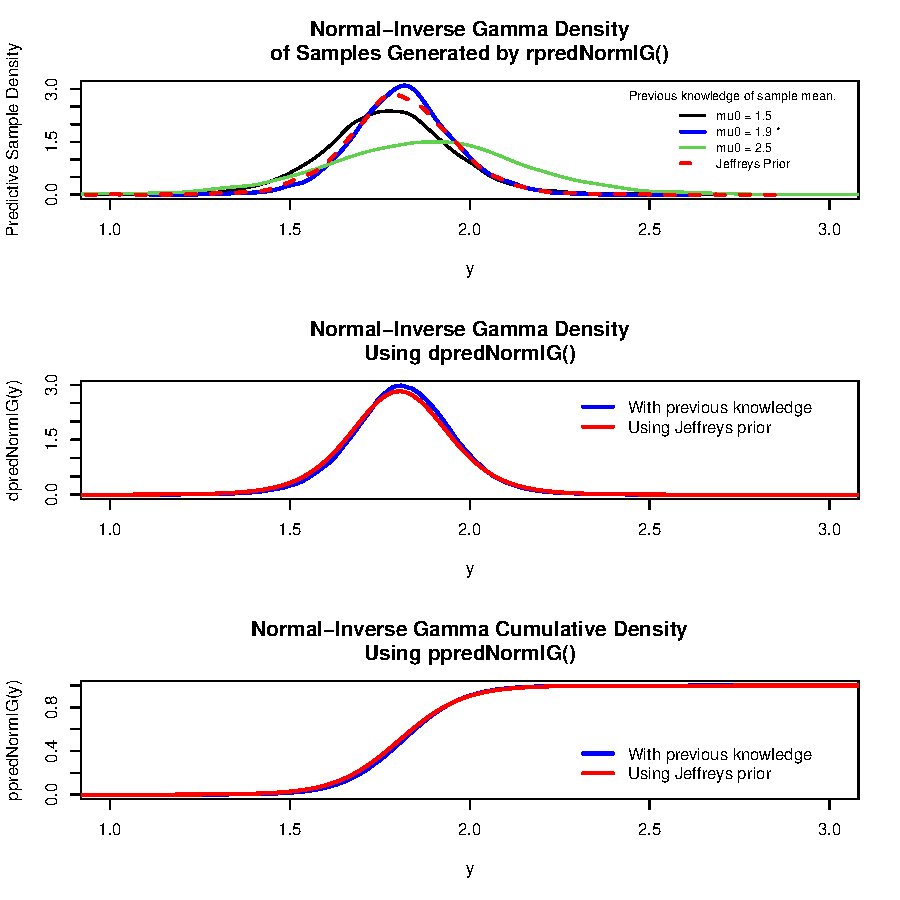
\includegraphics{Thesis-005}

        \clearpage

    \subsubsection{Two samples}
      \paragraph{Derivation}
      \paragraph{R Implementation}
      \paragraph{Example}
    \subsubsection{$k$ samples}
      \paragraph{Derivation}
      \paragraph{R Implementation}
      \paragraph{Example}
      \paragraph{Ranking Treatments}

\clearpage


\section{Chapter 2:  Normal Regression with Zellner's $g$-prior}
  \paragraph{Derivation}
  \paragraph{R Implementation}
  \paragraph{Example}


\clearpage

\section{Conclusion}

\end{document}
